\chapter{Ergebnisse} \label{ch:results}

\section{\acs{icd10gm} in der \acs{csv}-Dateien und \acs{db}} \label{sec:dataanalysis}
Die Analyse der Information der \ac{icd10gm} wurde mit Hilfe von \ac{sql}-Befehlen und der Skript Sprache Python unter dem Framework Jupyter-Notebook durchgeführt.

Wie in der Tabelle~\ref{tab:icdfiles} dargestellt wird, jede Kode-Datei enthält mehr als 15450 Kodes, obwohl manche Kodierungen gelöscht werden, nimmt die Menge neuer \ac{icd10gm} ständig zu.

\begin{table}[ht]
	\centering
	\small
	\caption[\acs{icd10gm} in den \acs{csv}-Dateien]{Anzahl an \acs{icd10gm} pro Jahr in den \ac{csv}-Dateien}
	\label{tab:icdfiles}
	\begin{tabular}{|l|l|}
		\hline
	\rowcolor{lightgray} Anzahl & Fassung \\ \hline 
		15455 & 2007 \\ \hline
		15498 & 2008 \\ \hline
		15523 & 2009 \\ \hline
		15598 & 2010 \\ \hline
		15633 & 2011 \\ \hline
		15643 & 2012 \\ \hline
		15668 & 2013 \\ \hline
		15688 & 2014 \\ \hline
		15761 & 2015 \\ \hline
		15821 & 2016 \\ \hline
		15930 & 2017 \\ \hline
		16059 & 2018 \\ \hline
		16126 & 2019 \\ \hline
		16131 & 2020 \\ \hline
		16203 & 2021 \\ \hline
		\hline
		236737 & \textbf{Gesamt} \\ \hline
	\end{tabular}
	\end{table}

Nach dem Durchlauf der \ac{etl} sind insgesamt 16520 \ac{icd10gm} von 2007 bis 2021 in der \ac{db} eingefügt. In der Abbildung~\ref{fig:icddb} ist das Verhältnis dieser Kodierungen in Bezug auf die Modifikationen dargestellt. Die konkreten Zahlen dieser Modifikationen sind in der Tabelle~\ref{tab:icdupd} dargestellt. 
 
 \begin{figure}[ht]
 	\centering
 	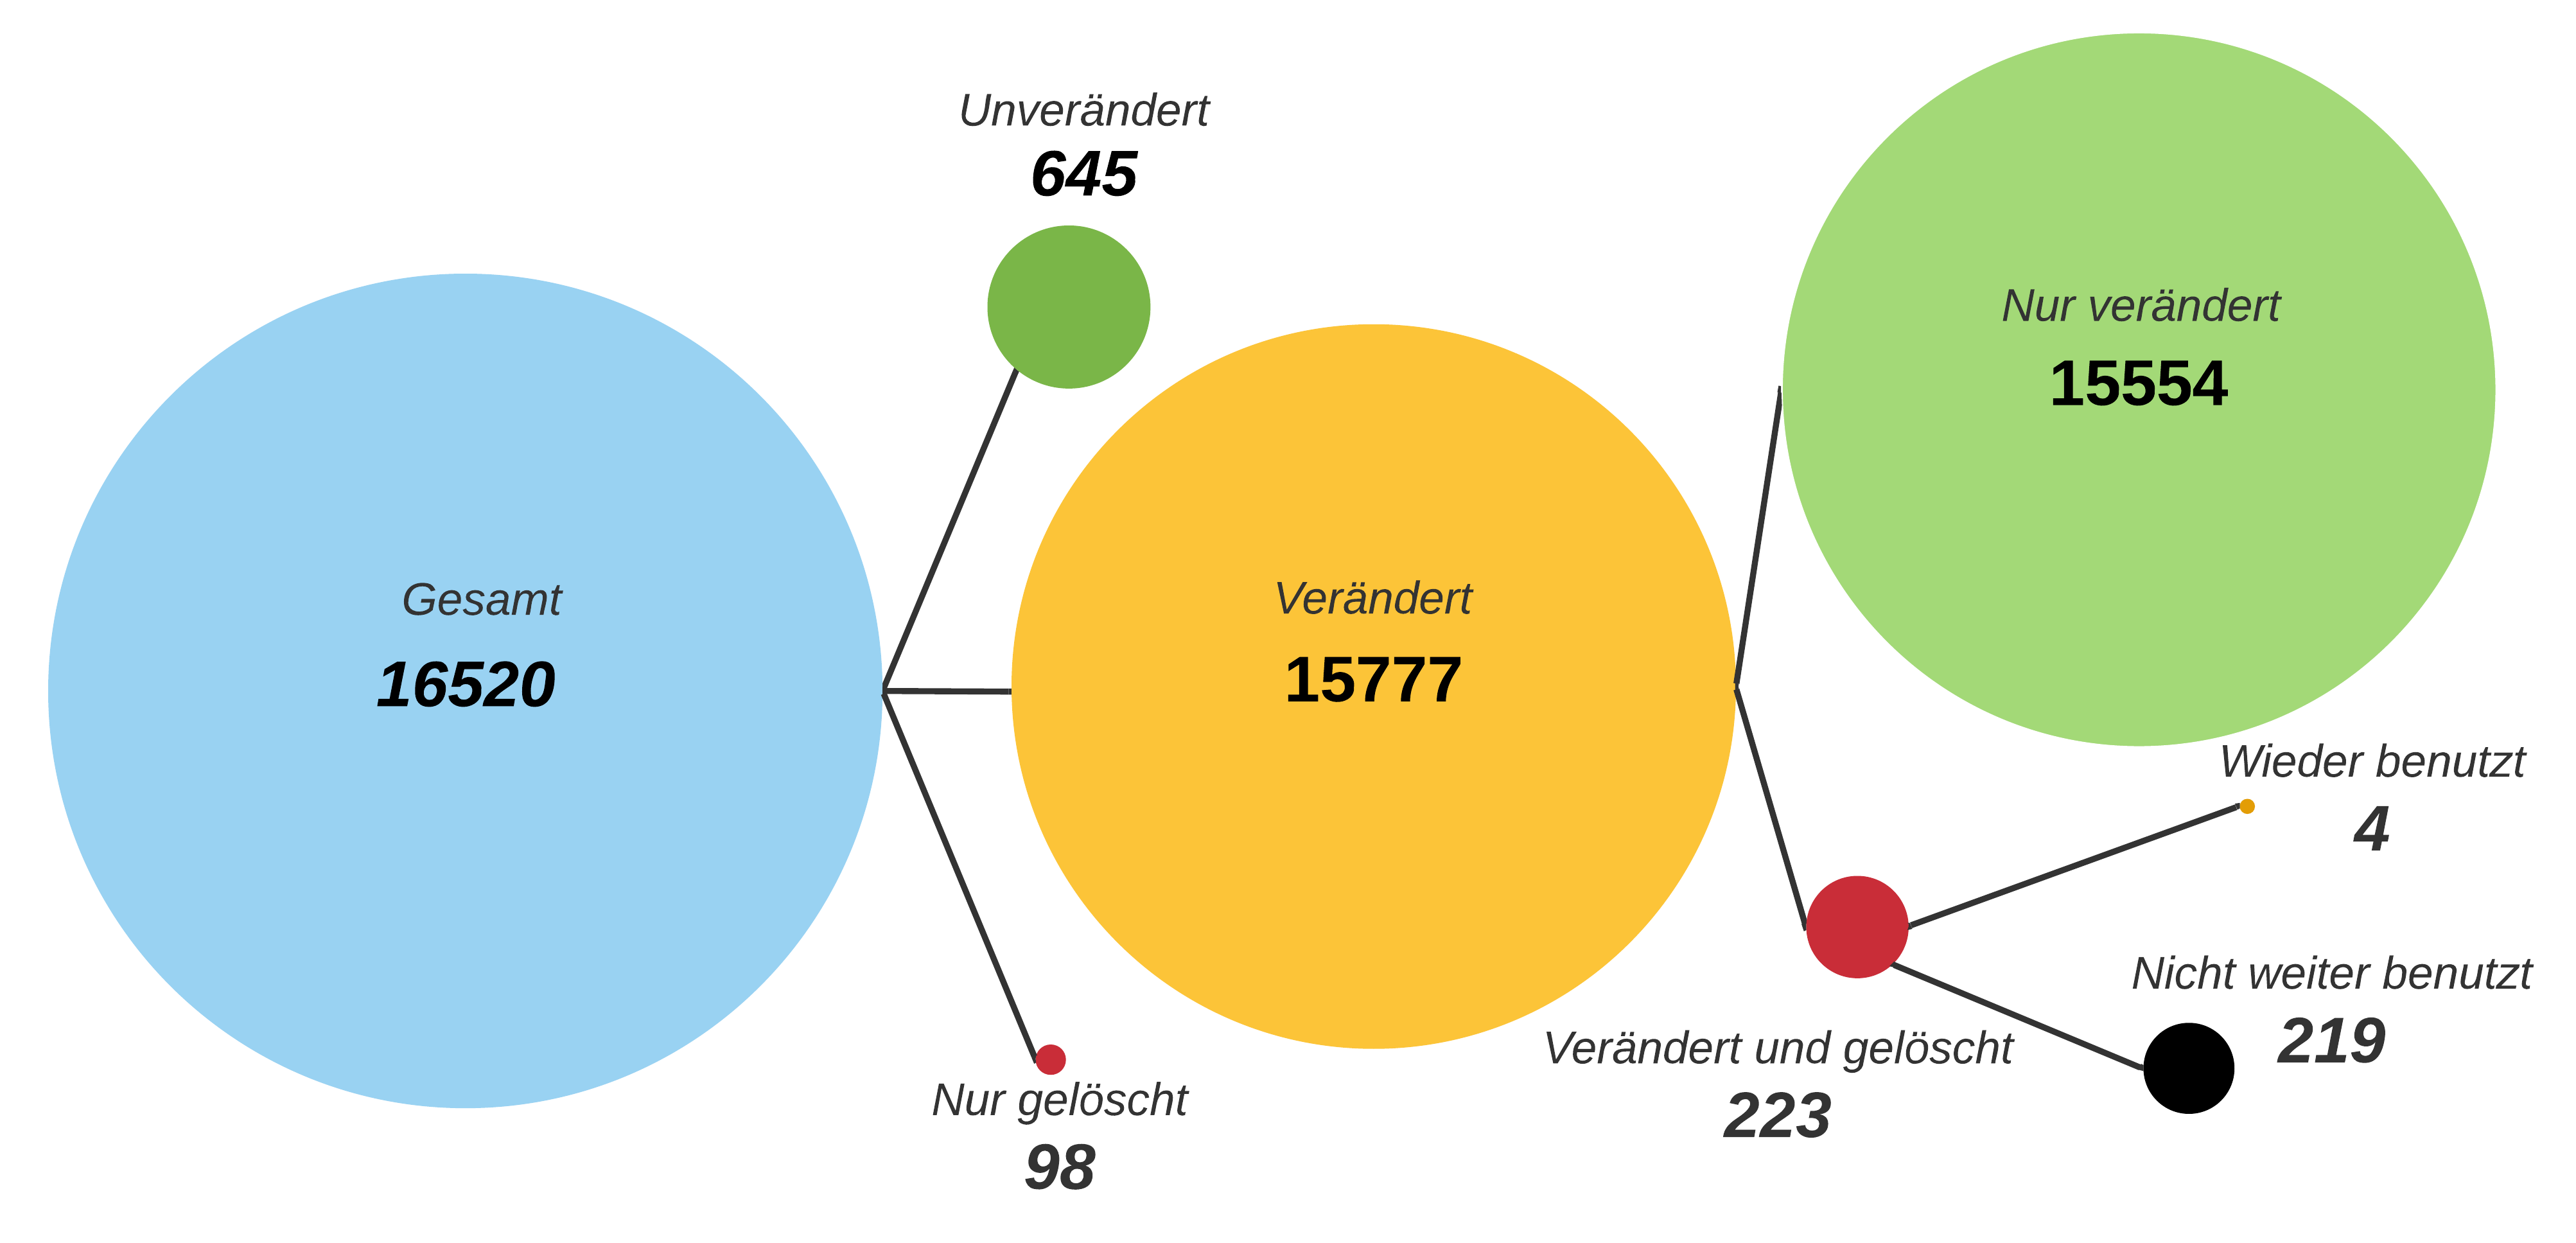
\includegraphics[height=6cm]{figures/icd10gm_quantities}
 	\caption[\acs{icd10gm} in der \acs{db}]{Charakterisierung der \acs{icd10gm} in der \ac{db} in Bezug auf die Modifikationen.}
 	\label{fig:icddb}
 \end{figure}

\section{Zeitliche Entwicklung der \acs{icd10gm}} \label{sec:timeicd}

Die Darstellung der Besonderheiten eines Lebenszyklus der historischen \ac{icd10gm} Auffassungen ist in der Tabelle~\ref{tab:IUDDI} exemplarisch dargestellt. Das Beispiel zeigt die chronologische Entwicklung der \ac{icd10gm} in der Tabelle \glqq\textsf{icd10gm\_history}\grqq{} der \ac{db}. Die Spalte Fassung, \glqq\textsf{ver}\grqq{} in der Tabelle \glqq\textsf{icd10gm\_history}\grqq{}, zeigt die Version der Einführung, Änderung, Löschung oder Wiederverwendung einer \ac{icd10gm}. Das Feld Alte Fassung, \glqq\textsf{oldver}\grqq{} in der vorher genannten Tabelle, beinhaltet den Identifikator der vorherigen Fassung einer Schlüsselnummer. In der Spalte Ereignis, \glqq\textsf{verevent}\grqq{} in der Tabelle \glqq\textsf{icd10gm\_history}\grqq{}, sind die Ereignisse Einführung, Änderung, Löschung und Wiederverwendung, wie in der Subsektion~\ref{subsec:newtables} beschrieben wurden, kodiert. Eine wichtige Anmerkung in der Darstellung ist, dass die gezeigte alte Fassung bei der wiederverwendeten Klassifikationen, die Version der Insertion oder der letzten Änderung ist, weil dieser Kode in der Fassung der Löschung nicht vorhanden war.

Somit könnten wir erkennen, dass unsere Implementierung die Lebenszyklus von \ac{icd10gm} Klassifikationen darstellen kann, sodass jede Modifikation in der Semantik zwischen 2007 und 2021 dokumentiert ist. In den weiteren Sektionen werden die verschiedenen Änderungen in dem semantischen Verzeichnis und einigen Sonderverzeichnissen gezeigt und deren Gründe erklärt.
%\clearpage

\begin{table}[ht]
	\centering
	\small
	\caption[Beispiel der Historisierung einer \acs{icd10gm} Klassifikation]{Beispiel der Historisierung einer \acs{icd10gm} Klassifikation. Diese stellt eine, nach der Einführung, veränderte, gelöschte, und wieder benutzte Schlüsselnummer dar.}
	\label{tab:IUDDI}
	\begin{tabular}{|l|l|p{6cm}|l|l|}
		\hline
		\rowcolor{lightgray} Fassung & Kode & Titel & Alte Fassung & Ereignis \\ \hline
		2007 & N90.8  & Sonstige näher bezeichnete nichtentzündliche Krankheiten der Vulva und des Perineums &  & I \\ \hline
		2008 & N90.8  & Sonstige näher bezeichnete nichtentzündliche Krankheiten der Vulva und des Perineums & 2007 & U \\ \hline
		2013 & N90.8  & Sonstige näher bezeichnete nichtentzündliche Krankheiten der Vulva und des Perineums & 2008 & U \\ \hline
		2014 & N90.8  & Sonstige näher bezeichnete nichtentzündliche Krankheiten der Vulva und des Perineums & 2013 & D \\ \hline
		2016 & N90.8  & Sonstige näher bezeichnete nichtentzündliche Krankheiten der Vulva und des Perineums & 2013 & DI \\ \hline
	\end{tabular}
\end{table}

\section{Neue \acs{icd10gm}} \label{sec:newicd}

Von 2008 bis 2021 sind insgesamt 966 neue \ac{icd10gm} entstanden. In der Abbildung~\ref{fig:newicdyear} ist ein interessanter Aspekt davon repräsentiert, nämlich die Anzahl neuer \ac{icd10gm} pro Jahr ist unregelmäßig. Es gib Jahre wie 2017 und 2018 mit mehr als 120 neuen Einträgen. Dieses Phänomen passiert am meisten beim Bedarf neuer Subklassifikationen, um die Diagnosen spezifischer zu kodieren und an diverse klinische Systeme anzupassen. Ein Beispiel dieses Phänomens ist der Kode \textsf{U81!} \textsf{Bakterien mit Multiresistenz gegen Antibiotika}, dieser wurde 2017 entnommen und stattdessen entstand die Kodierung \textsf{U81.-!} \textsf{Gramnegative Erreger mit bestimmten Antibiotikaresistenzen, die besondere therapeutische oder hygienische Maßnahmen erfordern} zusammen mit 43 weiteren Subklassifikationen von \textsf{U81.0-!} bis \textsf{U81.8!}. Die Ursache davon war eine Umstrukturierung der Bereiche \textsf{U81!}, um diese Kodes an die Nomenklatur der \ac{krinko} anzupassen~\cite{erreg17}.

Im Jahr 2018 wurden mehr als 80 neue \ac{icd10gm} in den Bereichen \textsf{M14.-*} \textsf{Arthropathien bei sonstigen anderenorts klassifizierten Krankheiten} eingefügt. Diese Zunahme ist auch in der Abbildung~\ref{fig:newicdcap} widerspiegelt, denn diese Diagnosen sind im Kapitel \textsf{Krankheiten des Muskel-Skelett-Systems und des Bindegewebes} repräsentiert. Die Ursache dieser Zunahme war die Insertion einer fünften Stelle an der Kodierung, um die Abbildung im \ac{gdrg}-System zu ermöglichen~\cite{musk18}.

%\clearpage

\begin{figure}[ht]
	\centering
	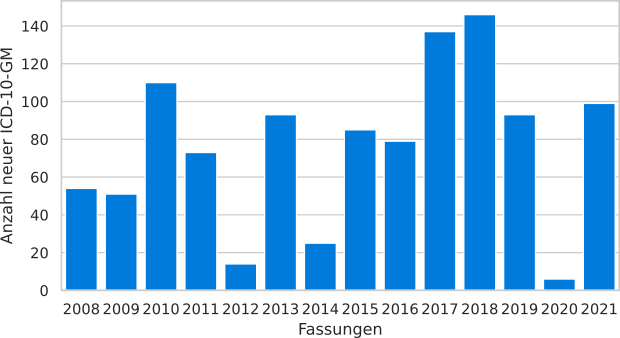
\includegraphics[height=7cm]{figures/newicdyear}
	\caption[Neue \acs{icd10gm} pro Jahr]{Anzahl neuer \acs{icd10gm} zwischen den Jahren 2008 und 2021}
	\label{fig:newicdyear}
\end{figure} 

Ein wichtiger und aktueller Punkt sind die meldepflichtigen Krankheiten im Laufe der Jahre. Dieses Phänomen ist in der Abbildung~\ref{fig:newicdmeld} dargestellt. Es ist zu erkennen, dass neue meldepflichtige Kodes in den Jahren 2010, 2016 und 2021 definiert wurden (Tabelle~\ref{tab:meldung}). Einige Ursachen davon sind Pandemien und Epidemien wie die Influenza Varianten zwischen 2009 und 2010~\cite{influenza1, influenza2}, und jetzt aktuell seit Februar 2020 die Verbreitung des Corona Virus in Europa~\cite{corona1} mit deren gesundheitlichen Folgen~\cite{corona2}. Andere Gründe für neue Kodierungen sind vorgenommene Umstrukturierungen der Kodebereiche. Ein Beispiel davon sind die Bereiche für Dengue. Diese wurden von der \ac{who}, 2016, umstrukturiert, und die dreistelligen Schlüsselnummern \textsf{A90} und \textsf{A91} wurden gestrichen und deren Inhalte in den neuen Kodebereich \textsf{A97.-} verlagert und auf vierstellige Subkategorien ausdifferenziert \cite{komm16}.

%die Verbreitung des Dengue Fiebers in Europa als Effekt der Globalisierung mit der steigenden Mobilität~\cite{denge1} und Verbreitung der asiatischen Tigermücke \textsl{Aedes (Stegomyia) albopictus} zwischen 2015 und 2016 in der Region als Konsequenz der milden Winter~\cite{denge2},

Ein interessanter Aspekt der meldepflichtigen Krankheiten in der Tabelle~\ref{tab:meldung} ist die Diagnose \textsf{B17.9} \textsf{Akute Virushepatitis, nicht näher bezeichnet}. Diese Krankheit war unter \textsf{K72.0} \textsf{Akutes und subakutes Leberversagen} zugeordnet, erst 2010 wurde zur Kenntnis genommen, dass es sich bei der akuten Hepatitis in manchen Fällen um eine akute infektiöse Hepatitis handelt. Aus diesem Grund hatte die \ac{who} die Schlüsselnummer \textsf{B17.9} zur Verfügung gestellt~\cite{komm10}.

\clearpage

\begin{figure}[ht]
	\centering
	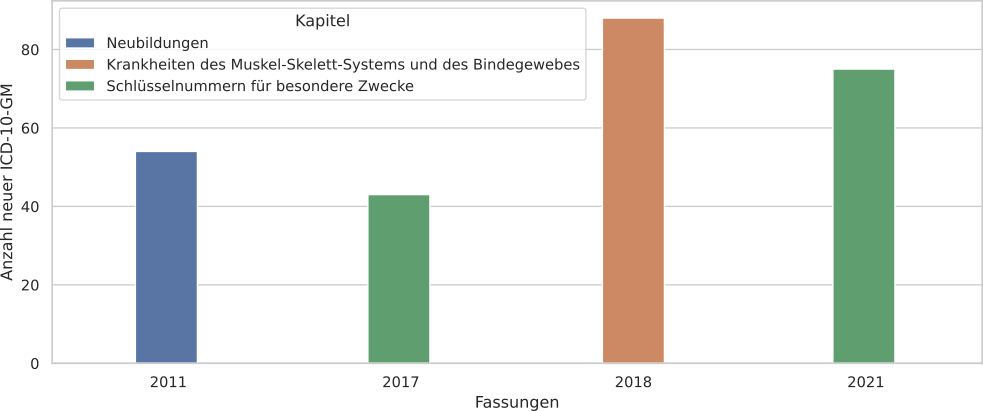
\includegraphics[height=5.7cm]{figures/kaptnrYear}
	\caption[Kapitel mit den meisten eingeführten \acs{icd10gm} (2008 - 2021)]{Kapitel mit den meisten neuen Kodierungen zwischen 2008 und 2021}
	\label{fig:newicdcap}
\end{figure}

%\clearpage
\begin{figure}[ht]
	\centering
	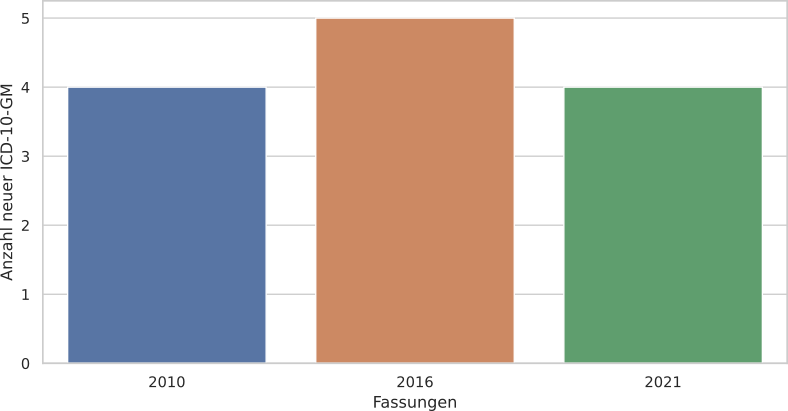
\includegraphics[height=5.7cm]{figures/arztJaYear}
	\caption[Neue meldepflichtige \acs{icd10gm} pro Jahr]{Menge der neuen meldepflichtigen Diagnosen zwischen den Jahren 2008 und 2021}
	\label{fig:newicdmeld}
\end{figure} 

\clearpage
\begin{table}[ht]
	\centering
	\small
	\caption[Meldepflichtige \acs{icd10gm}]{Meldepflichtige Krankheiten}
	\label{tab:meldung}
	\begin{tabular}{|l|l|p{10.5cm}|}
		\hline
		\rowcolor{lightgray} Fassung & \acs{icd10gm} & Titel \\ \hline
		2010 & B17.9 & Akute Virushepatitis, nicht näher bezeichnet \\ \hline
		2010 & U69.2-! & Sekundäre Schlüsselnummern für besondere epidemiologische Zwecke \\ \hline
		2010 & U69.20! & Influenza A/H1N1 Pandemie 2009 [Schweinegrippe] \\ \hline
		2010 & U69.21! & Influenza A/H5N1 Epidemie [Vogelgrippe] \\ \hline
		2016 & A97.- & Dengue \\ \hline
		2016 & A97.0 & Dengue ohne Warnzeichen \\ \hline
		2016 & A97.1 & Dengue mit Warnzeichen \\ \hline
		2016 & A97.2 & Schweres Dengue \\ \hline
		2016 & A97.9 & Dengue, nicht näher bezeichnet \\ \hline
		2021 & U07.1! & COVID-19, Virus nachgewiesen \\ \hline
		2021 & U07.2! & COVID-19, Virus nicht nachgewiesen \\ \hline
		2021 & U10.- & Multisystemisches Entzündungssyndrom in Verbindung mit COVID-19 \\ \hline
		2021 & U10.9 & Multisystemisches Entzündungssyndrom in Verbindung mit COVID-19, nicht näher bezeichnet \\ \hline
	\end{tabular}
\end{table}

\section{Modifizierte \acs{icd10gm}} \label{sec:updicd}

Jedes Jahr werden Änderungen in den Metadaten der \ac{icd10gm} vorgenommen. Solche Modifikationen sind in der Tabelle \ref{tab:icdupd} aufgelistet. Wie in der Sektion~\ref{sec:dataanalysis} genannt wurde, sind die meisten Änderungen an den Spalten für die dritten, vierten und fünften Stellen  der Kodes, weil diese Felder erst im Jahr 2013 entstanden sind~\cite{readme13}. Ein weiterer Aspekt in Bezug auf die zahlreichen Änderungen ist, dass die Werte verschiedener Felder bei manchen \ac{icd10gm} in früheren Fassungen noch nicht definiert waren, wie in der Tabelle~\ref{tab:icdupd} in den Fällen der Mortaliätslisten verdeutlicht wird. Die Werte solcher Listen bei den meisten Kodes im Jahr 2007 waren nicht definiert, und waren mit dem Wert \glqq\textsf{UNDEF}\grqq{} gesetzt. Erst 2008 wurden diese Felder durch einen spezifischen Wert ersetzt. Die zahlreichen Modifikationen an den Klassentiteln sind durch Vorschläge zur Weiterentwicklung der Klassifikationen entstanden~\cite{diab09, komm14}. 
%  Ein Beispiel davon ist die Schlüsselnummer \textsf{E10.31} mit dem Titel \textsf{Primär insulinabhängiger Diabetes mellitus [Typ-1-Diabetes] \underline{mit} Augenkomplikationen: Als entgleist bezeichnet}. Dieser Titel wurde zu \textsf{Primär insulinabhängiger Diabetes mellitus [Typ-1-Diabetes] \underline{: Mit } Augenkomplikationen: Als entgleist bezeichnet} in 2009 geändert. Die Änderung wurde in diesem Jahr durchgeführt, da eine fünfte Stelle in der Klassifikationen von \textsf{E10}  bis \textsf{E14} eingefügt wurde~\cite{diab09}. Der Titel dieser \ac{icd10gm} wurde nochmal in 2014 zu \textsf{\underline{Diabetes mellitus, Typ 1: Mit Augenkomplikationen: Als entgleist bezeichnet}} ersetzt. In diesem Jahr wurden die Titel von der \ac{who} an die gebräuchliche Terminologie angepasst~\cite{komm14}.

%\clearpage

\begin{table}[ht]
	\centering
	\small
	\caption[Änderungen in den Metadaten]{Liste der Metadaten und Anzahl an Änderungen}
	\label{tab:icdupd}
	\begin{tabular}{|l|p{11.5cm}|}
		\hline
		\rowcolor{lightgray} Änderungen & Metadaten \\ \hline
		15578 & Dritte Stelle \\ \hline
		13871 & Vierte Stelle \\ \hline
		6949 & Bezug zur Mortalitätsliste 3 \\ \hline		
		6348 & Bezug zur Mortalitätsliste 1 \\ \hline
		2 & \textbf{Bezug zur Mortalitätsliste 1 (definiert)} \\ \hline
		5061 & Fünfte Stelle \\ \hline
		%1193 & Art des Fehlers bei Geschlechtsbezug \\ \hline
		1111 & Klassentitel \\ \hline
		308 & Untere Altersgrenze \\ \hline
		36 & \textbf{Untere Altersgrenze (relevant)} \\ \hline
		299 & Bezug zur Morbiditätsliste \\ \hline
		11 & \textbf{Bezug zur Morbiditätsliste (definiert)} \\ \hline
		%286 & Alter Fehlertyp \\ \hline
		286 & Obere Altersgrenze \\ \hline
		14 & \textbf{Obere Altersgrenze (relevant)} \\ \hline
		162 & Anwendung der Laborausschlussziffer des \ac{ebmg} \\ \hline
		118 & Art der Vier- und Fünfsteller \\ \hline
		69 & Bezug zur Mortalitätsliste 4 \\ \hline
		68 & Geschlechtsbezug \\ \hline
		64 & Bezug zur Mortalitätsliste 2 \\ \hline
		2 & \textbf{Bezug zur Mortalitätsliste 2 (definiert)} \\ \hline
		44 & Kategorie der Gruppe \\ \hline
		40 & Arzt-Meldepflicht \\ \hline		
		31 & Sehr seltene Krankheit in Mitteleuropa \\ \hline				
		6 & Belegung des Kodes \\ \hline
		3 & \S 295 \ac{sgb} V \\ \hline		
		2 & Klassifikationsebene \\ \hline
		
	\end{tabular}
\end{table}

Ein interessanter Aspekt an der Stelle des Geschlechtsbezugs ist, dass 52 Diagnosen mit Geschlechtsbezug der 68 an dieser Stelle geänderten Schlüsselnummer, Krankheiten der Brustdrüse sind. Diese \ac{icd10gm} waren früher auf das weibliche Geschlecht bezogen, jetzt ist der Geschlechtsbezug dieser Kodierungen irrelevant. Viele dieser Änderungen wurden in den Jahren 2008 und 2016 vorgenommen. An dieser Stelle können wir nicht erklären, wieso diese Art von Krankheiten nicht immer ohne Geschlechtsbezug waren, denn seit 1930 existieren medizinische Publikationen über Brustdrüsen Anomalien bei Männern~\cite{bcm}. In den heutigen Tagen gibt es eine leichte Zunahme an Männern mit Brustkrebs~\cite{giobcm} und die erste deutschsprachige Fassung der ICD-10 für die Zwecke des \ac{sgb} V wurde schon 1996 erarbeitet~\cite{icdgmhistory}.

\clearpage

\begin{table}[ht]
	\centering
	\caption[Beispiel von seltenen Krankheiten in Mitteleuropa (Diphtherie und Poliomyelitis)]{Beispiel von seltenen Krankheiten in Mitteleuropa anhand von \ac{icd10gm} der Bereiche \textsf{A36.-} \textsf{Diphtherie} und \textsf{A80.-} \textsf{Akute Poliomyelitis [Spinale Kinderlähmung]}. Die alten und neuen Werte sind in der Spalte \glqq Alt\grqq{} bzw. \glqq Neu\grqq{}. \glqq\textsf{N}\grqq{} Nein, \glqq\textsf{J}\grqq{}\grqq{} Ja.}
	\label{tab:icdeuropa}
	\begin{tabular}{|p{1.6cm}|l|p{7cm}|l|l|}
		\hline
		\rowcolor{lightgray} Fassung der Änderung & \ac{icd10gm} & Titel & Alt & Neue \\ \hline
		\rowcolor{maroon!10} 2011 & A36.- & Diphtherie & N & J \\ \hline
		2011 & A36.0 & Rachendiphtherie & N & J \\ \hline
		2011 & A36.1 & Nasenrachendiphtherie & N & J \\ \hline
		2011 & A36.2 & Kehlkopfdiphtherie & N & J \\ \hline
		2011 & A36.3 & Hautdiphtherie & N & J \\ \hline
		2011 & A36.8 & Sonstige Diphtherie & N & J \\ \hline
		2011 & A36.9 & Diphtherie, nicht näher bezeichnet & N & J \\ \hline \hline
		\rowcolor{maroon!10} 2011 & A80.- & Akute Poliomyelitis [Spinale Kinderlähmung] & N & J \\ \hline
		2011 & A80.0 & Akute paralytische Poliomyelitis durch Impfvirus & N & J \\ \hline
		2011 & A80.1 & Akute paralytische Poliomyelitis durch importiertes Wildvirus & N & J \\ \hline
		2011 & A80.2 & Akute paralytische Poliomyelitis durch einheimisches Wildvirus & N & J \\ \hline
		2011 & A80.3 & Sonstige und nicht näher bezeichnete akute paralytische Poliomyelitis & N & J \\ \hline
		2011 & A80.4 & Akute nichtparalytische Poliomyelitis & N & J \\ \hline
		2011 & A80.9 & Akute Poliomyelitis, nicht näher bezeichnet & N & J \\ \hline
	\end{tabular}
\end{table}

Von den sehr seltenen Krankheiten in Mitteleuropa sind 20 der 31 Diagnosen belegte Schlüsselnummern, also Kodierungen ohne Unterkategorien und somit im alltäglichen  Gebrauch. Davon gehören 12 zu den Bereichen \textsf{A36.-} \textsf{Diphtherie} und \textsf{A80.-} \textsf{Akute Poliomyelitis [Spinale Kinderlähmung]}. Diese sind in der Tabelle~\ref{tab:icdeuropa} aufgelistet. Diese Diagnosen sind heutzutage selten, Ursache ist die erfolgreiche Impfkampagne in Deutschland, sodass die vom \ac{rki} jährlich selten gemeldeten Fällen in den heutigen Tagen importiert sind~\cite{dippol1}.

\section{Gelöschte \acs{icd10gm}} \label{sec:deletedicd}

In jeder Fassung von 2008 bis 2021 werden \ac{icd10gm} gelöscht. Dieses Verhalten ist in der Abbildung~\ref{fig:newdeleteoldicdyear} repräsentiert. Die meisten Schlüsselnummern wurden im Jahr 2013 gelöscht, da eine umfangreiche Umstrukturierung in der Semantik in diesem Jahr vorgenommen wurde. Die Kapitel, die in diesem Jahr am meisten betroffen waren, sind in der Abbildung~\ref{fig:kap13} dargestellt. Bei der semantischen Umstrukturierung im Jahr 2013 wurden bestimmte Kodebereiche im Kapitel \textsf{Krankheiten des Kreislaufsystems} umfänglich überarbeitet, viele fünfstellige Klassifizierungen wurden vom Kapitel \textsf{Krankheiten des Muskel-Skelett-Systems und des Bindegewebes} entnommen, und im Kapitel \textsf{Schlüsselnummern für besondere Zwecke} wurden zahlreiche \ac{icd10gm} umgebaut~\cite{dele13}.

%\clearpage
\begin{figure}[ht]
	\centering
	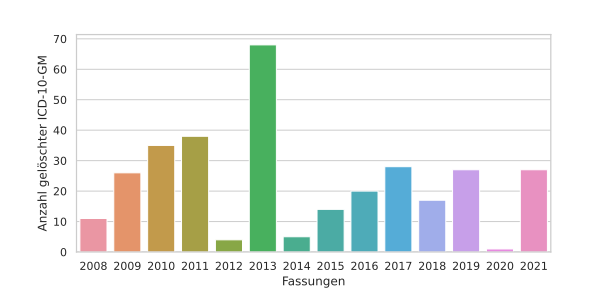
\includegraphics[height=6cm]{figures/neuVersionDelete}
	\caption[Gelöschte \acs{icd10gm} pro Jahr]{Anzahl gelöschter \acs{icd10gm} zwischen den Jahren 2008 und 2021}
	\label{fig:newdeleteoldicdyear}
\end{figure} 

\clearpage

\begin{figure}[ht]
	\centering
	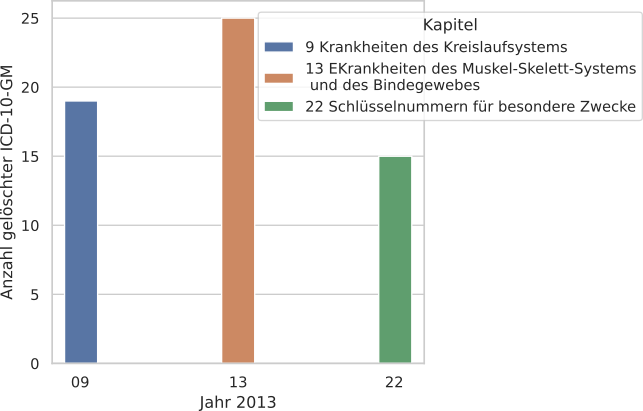
\includegraphics[height=6cm]{figures/kaptnr13}
	\caption{Meist betroffene Kapitel beim Löschen 2013}
	\label{fig:kap13}
\end{figure}


Die Abbildung \ref{fig:oldicdort} zeigt, dass die meisten Kodes, nämlich 295 der 321 gelöschten Kodierungen, terminale Schlüsselnummer waren, also \ac{icd10gm}, die in den Texten der Dokumentation der Diagnosen benutzt werden sollen. Von diesen terminalen Kodierungen wurden 115 erweitert, wie in der Sektion \ref{sec:newicd} Anhang des Beispiels von \textsf{U81!} erläutert wurde. Von den nicht terminalen Kodierungen wurden dann 11 erweitert. Ein Beispiel davon ist \textsf{Z75.2-} \textsf{Wartezeit auf eine Untersuchung oder Behandlung}. Diese nicht terminale Kodierung wurde gelöscht, und von dem terminalen Kode \textsf{Z75.2} mit demselben Titel ersetzt. 

%\clearpage

\begin{figure}[ht]
	\centering
	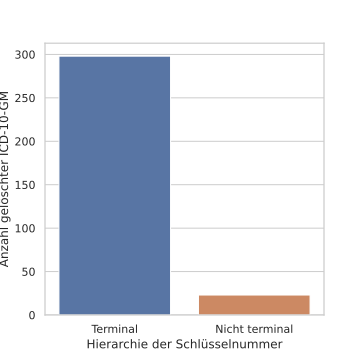
\includegraphics[height=6cm]{figures/ortoldYear}
	\caption{Hierarchie der gelöschten \acs{icd10gm}}
	\label{fig:oldicdort}
\end{figure}

%\newpage

\section{Wiederverwendete \acs{icd10gm}} \label{sec:delinicd}

Ein unerwartetes Phänomen dieser Projektarbeit war die Erkennung von wiederverwendeten Kodierungen. Die Tabelle~\ref{tab:wieder} zeigt die 4 wiederverwendeten Schlüsselnummern.

\begin{table}[ht]
	\centering
	\small
	\caption[Wieder benutzte \acs{icd10gm}]{Liste der wieder benutzten Schlüsselnummern.}
	\label{tab:wieder}
	\begin{tabular}{|l|l|l|p{6cm}|}
		\hline
		\rowcolor{lightgray} Gelöscht & Wieder & \ac{icd10gm} & Aktueller Titel \\ \hline
		2013 & 2015 & M21.60 & Erworbener Hohlfuß [Pes cavus] \\ \hline
		2013 & 2015 & M21.6- & Sonstige erworbene Deformitäten des Knöchels und des Fußes \\ \hline
		2014 & 2016 & N90.8 & Sonstige näher bezeichnete nichtentzündliche Krankheiten der Vulva und des Perineums \\ \hline
		2010 & 2019 & K55.8 & Sonstige Gefäßkrankheiten des Darmes \\ \hline

\end{tabular}
\end{table}

Die Schlüsselnummern \textsf{M21.6-} und \textsf{M21.60} wurden 2013 entnommen, da im Kodebereich \textsf{M20-M25} zahlreiche Schlüssel zu keinen sinnvollen Kombinationen führten~\cite{dele13}. Andererseits wurde 2015 die Kategorie \textsf{M21.6} mit den genannten Schlüsselnummern wieder aufgenommen, um eine bessere Spezifikation der Diagnosen in dem \ac{gdrg}-System zu erreichen~\cite{komm15}. 

Die \ac{icd10gm} \textsf{N90.8} wurde 2014 entnommen und stattdessen wurde \textsf{N90.8-} \textsf{Sonstige näher bezeichnete nichtentzündliche Krankheiten der Vulva und des Perineums} mit weiteren Subklassifikationen zur spezifischen Kodierung eingeführt~\cite{komm14}. Zwei Jahre später, 2016, wurde der Kode \textsf{N90.8-} und deren Unterkategorien wieder entnommen und zu einem anderen Kapitel mit neuen Kodierungen verlagert, und die Schlüsselnummer \textsf{N90.8} wurde wieder eingeführt~\cite{komm16}.

Die Kodierungsschlüssel \textsf{K55.8} wurde 2010 gelöscht und die Kodierung \textsf{K55.8-} \textsf{Sonstige Gefäßkrankheiten des Darmes} mit weiteren Stellen eingeführt, um einige Diagnosen des Dünndarms besser abgrenzen zu können~\cite{komm10}. 2019 wurde die \ac{icd10gm} \textsf{K55.3-} \textsf{Angiodysplasie des Dünndarmes} mit weiteren fünfstelligen Kodes eingeführt und die, 2010, eingeführten Klassifikationen wurden auf den neuen Kodebereich verlagert, sodass die Kodierungen von 2010 obsolet wurden, und \textsf{K55.8} wieder benutzt wurde~\cite{komm19}.

\section{Strukturelle Änderungen} \label{sec:strucmodif}

Wie in der Subsektion \ref{subsec:transf} genannt wurde, gab es auch Änderungen in der Struktur des semantischen Verzeichnisses. Im Jahr 2013 wurde die Spalte \glqq\textsf{titel}\grqq{} für den Klassentitel der Tabelle \glqq\textsf{kodes}\grqq{} aus dem Dreisteller-, Viersteller- und gegebenenfalls Fünfstellertitel zusammengesetzt. Auch in diesem Jahr wurden drei neue Felder für die einzelnen Bestandteile des zusammengesetzten Klassentitels eingefügt~\cite{readme13}. Eine weitere Änderung in der Tabelle \glqq\textsf{kodes}\grqq{}, die schon seit 2015 geplant wurde, und im Jahr 2018 vorgenommen wurde, war die Entnahme der Felder der Altersklassenformate für die untere und obere Grenze des Altenbezuges mit Angabe von Tagen, Wochen, Monaten und Jahren; und damit blieben nur die Felder mit dem Format in Tagen und Jahren, nämlich  \glqq\textsf{altunt}\grqq{} für die untere Grenze und \glqq\textsf{altob}\grqq{} für die obere Grenze des Altenbezuges~\cite{readme17}.
